% This is samplepaper.tex, a sample chapter demonstrating the
% LLNCS macro package for Springer Computer Science proceedings;
% Version 2.21 of 2022/01/12
%
\documentclass[runningheads]{llncs}
%
\usepackage[T1]{fontenc}
% T1 fonts will be used to generate the final print and online PDFs,
% so please use T1 fonts in your manuscript whenever possible.
% Other font encondings may result in incorrect characters.
%
\usepackage{graphicx}
% Used for displaying a sample figure. If possible, figure files should
% be included in EPS format.
%
% If you use the hyperref package, please uncomment the following two lines
% to display URLs in blue roman font according to Springer's eBook style:
%\usepackage{color}
%\renewcommand\UrlFont{\color{blue}\rmfamily}
%\urlstyle{rm}
%
\usepackage{graphicx}
\usepackage{float}
\begin{document}
%
\title{Módulo 3 ZZZ}
%
%\titlerunning{Abbreviated paper title}
% If the paper title is too long for the running head, you can set
% an abbreviated paper title here
%
\author{Maia Ortiz\inst{1}\orcidID{ } \and
Celina Lopez\inst{1}\orcidID{ } \and
Rocio Gomez\inst{1}\orcidID{ } \and
Bautista Pons\inst{1}\orcidID{ }}
%
\authorrunning{B. Pons}
% First names are abbreviated in the running head.
% If there are more than two authors, 'et al.' is used.
%
\institute{Universidad Nacional de Cuyo, Instituto de Ingeniería Industrial \and
\email{baupons@gmail.com}\\
\url{http://ingenieria.uncuyo.edu.ar/} \and
%ABC Institute, Rupert-Karls-University Heidelberg, Heidelberg, Germany\\
%\email{\{abc,lncs\}@uni-heidelberg.de}}
}
%
\maketitle              % typeset the header of the contribution
%
\begin{abstract}
Este estudio analiza y optimiza un sistema de procesos mediante un modelo de simulación de eventos discretos en Simul8.
\keywords{Simulación de eventos discretos  \and Simul8  \and Optimización de procesos. }
\end{abstract}
%
%
%
\section{Programa SIMUL8}
A continuación se dará una descripción de los elementos que componen las barras de menú y estándar del programa

\subsection{Barra menú}
\begin{figure}[h]
    \centering
    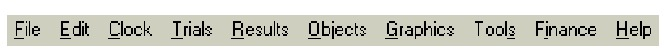
\includegraphics[width=0.65\textwidth]{Imagen 1.jpeg}
    \caption{Barra menú de Simul8}
    \label{fig:mi_imagen}
\end{figure}

Esta barra contiene los elementos básicos que contiene cualquier programa, tales como:\\

- \textbf{FILE}: Ejecuta las funciones de abrir una nueva hoja de Simul8, guardar, guardar como, imprimir, salir, cerrar, etc. En este menú, en Preferencias, se busca distancia y se activa “Zero”. \\

- \textbf{EDIT}: Realiza las funciones de deshacer, copiar, pegar, seleccionar todo y buscar nombres de los objetos.\\

- \textbf{CLOCK}: Las propiedades del reloj pueden ser cambiadas usando la barra de menú o haciendo doble click en la ventana del reloj. El reloj puede ser digital o análogo e ilustra la información referente al día y semana en que es llevada a cabo la simulación. En el cuadro de diálogo del reloj se fija la hora en que comienza la simulación (Start time each day), el tiempo simulado en cada día (Time in each day), al cabo de cuánto tiempo el sistema comienza a parecerse a la realidad y comienza la recolección de datos (Warm up period) y por cuanto tiempo se recolectarán los datos cuando corra la simulación. 

En el menú se ven los elementos: Run (corre la simulación), Stop (detiene la simulación), Reset to Start (reinicia la simulación y los resultados), Step (corre la simulación paso a paso), Monitor Simulation (monitorea la simulación, mostrando el historial de lo que está pasando en cada corrida y lo que pasará más adelante), Simulation Speed (controla la velocidad de la simulación). 

Algunas de las funciones que realiza el reloj se encuentran ubicadas también en la barra estándar. Las figuras correspondientes son: 

\begin{figure}[H]
    \centering
    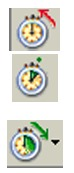
\includegraphics[width=0.15\textwidth]{Imagen 2.jpeg}
    \caption{\\ 1. Reset Clock to start\\ 2. Step \\ 3. Run (tiene la opción de correr el modelo con diferentes números aleatorios y con múltiples corridas)}
    \label{fig:mi_imagen}
\end{figure}

- \textbf{TRIALS}: Una prueba (trial) o experimento es una serie de corridas del modelo de simulación, el cual funciona con las mismas condiciones y parámetros, pero cambiando los números aleatorios. Dado que un modelo de simulación contiene variabilidad, es importante que este sea corrido más de una vez. En el cuadro de  diálogo Conduct Trials es posible ajustar el número de corridas en cada experimento, y en el cuadro Random Sampling se puede variar la semilla de la función aleatoria. \\

- \textbf{RESULTS}: Permiten recolectar y revisar las medidas de desempeño, las cuales predicen qué tan real es el comportamiento del sistema. Haciendo doble clic en el objeto sobre el cual se quieren ver los resultados o en “Resultados” en el menú principal y luego doble clic sobre el tipo de objeto, se despliega un cuadro de diálogo que contiene todas las medidas de desempeño que se pueden analizar. Haciendo clic derecho sobre los números de la parte derecha, se añaden las medidas que se desean. Se pueden realizar gráficos de tortas y del porcentaje de trabajo. Algunas medidas de desempeño son:  \\

1. \textit{Entrada}: Número de ítems que entran y que se pierden.

2. \textit{Cola}: Número de ítems en cola, tiempo promedio en cola (se analizan dos casos: considerando todos los ítems y considerando sólo aquellos que hicieron cola), porcentaje de ítems que esperaron menos de cierta cantidad de minutos. 

3. \textit{Servidor}: Número de ítems que pasaron por el centro de servicio, número total de trabajos completados, porcentaje de tiempo que el servidor está esperando porque no hay trabajo (Awaiting Work), porcentaje del tiempo que el servidor está parado porque otro no le manda trabajo (Blocked) y porcentaje del tiempo que el work center está parado porque hay paros de algún tipo o por eficiencia (Stopped). 

4. \textit{Salida}: Trabajos completados, tiempo en el sistema. 
\\

- \textbf{OBJECTS}: Se define el tipo de work ítem (elemento que fluye a través de la simulación), se pueden crear distribuciones, dar atributos a los ítems (labels), definir variables (information store), se pueden formar grupos con los objetos. \\

1. \textit{Labels}: es una característica que se le asigna a un ítem. Puede ser numérico o de texto y siempre debe ser adherido a éste. 

2. \textit{Information store}: permite crear variables y ver cómo cambian a través del tiempo. 

3. \textit{Distributions}: Simul8 permite trabajar con distribuciones estadísticas, tales como la Normal, Exponencial, etc., o diseñar una distribución propia, de modo que sea posible referirse a la misma distribución en varios lugares. 


\subsection{Barra Estándar} 

 Los elementos más importantes de la barra estándar son:

\begin{figure}[H]
    \centering
    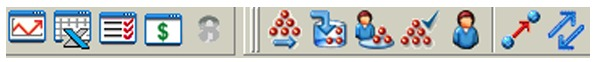
\includegraphics[width=0.5\textwidth]{Imagen 3.jpeg}
    \caption{}
    \label{fig:mi_imagen}
\end{figure}

\subsubsection{ENTRADA (WORK ENTRY POINT)}: La imagen es: 

\begin{figure}[H]
    \centering
    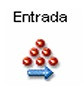
\includegraphics[width=0.15\textwidth]{Imagen 4.jpeg}
    \caption{}
    \label{fig:mi_imagen}
\end{figure}

La entrada es donde llegan los ítems. Se puede tener tantas entradas como sea necesario. Haciendo doble clic sobre ésta se despliega el siguiente cuadro de diálogo: 

\begin{figure}[H]
    \centering
    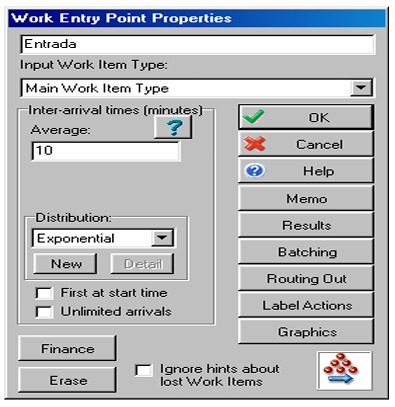
\includegraphics[width=0.5\textwidth]{Imagen 5.jpeg}
    \caption{}
    \label{fig:mi_imagen}
\end{figure}

- \textbf{Inter-arrival times} (Tiempo entre llegadas):  Aquí se selecciona la distribución con que llegan los ítems. Al seleccionarla, se deben introducir los parámetros requeridos. La distribución puede ser cualquiera de la lista o se puede crear una nueva (New).  \\

- \textbf{First at start time}: Si se selecciona esta opción, al inicio de la simulación, en el tiempo cero, llegará un ítem. \\

- \textbf{Unlimited Arrivals}: Esta opción sirve para que el ítem llegue exactamente cuando es requerido. \\

- \textbf{Memo}: permiten adicionar notas y documentación sobre cualquier objeto en la Simulación. \\

- \textbf{Resultados}: Muestran las medidas de desempeño que han sido recolectadas durante la corrida. \\

- \textbf{Batching} (Por lotes): El Batching permite la entrada de Work Ítems en grupos o lotes. El tiempo entre los lotes es definido en el Inter- arrival times. El número de ítems en un lote puede ser determinado por una distribución.  \\

- \textbf{Routing Out} (Ruta de Salida): Indica cómo debe salir el ítem hacia la próxima estación de trabajo en el proceso. Al hacer clic sobre éste se despliega el cuadro: 

\begin{figure}[H]
    \centering
    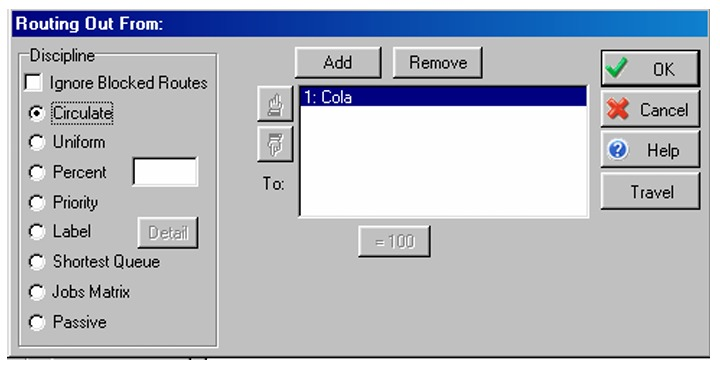
\includegraphics[width=0.5\textwidth]{Imagen 6.jpeg}
    \caption{}
    \label{fig:mi_imagen}
\end{figure}

 Al activar “Ignore Blocked Routes” Simul8 permite ignorar cualquier ruta que no esté disponible, por ejemplo cuando la cola no tiene más capacidad. Si no está activada esta opción, Simul8 espera hasta que la ruta esté disponible. \\
 
 - \textit{Circulate}: Cuando la entrada entrega ítems a varias estaciones, esta opción envía el primer ítem al primer destino en la lista, el segundo al segundo destino, y así sucesivamente hasta llegar al último destino de la lista, donde vuelve y empieza a enviar ítems al primer destino. Esta opción está seleccionada por defecto.
 
 - \textit{Uniform}: El work ítem es distribuido aleatoriamente con igual probabilidad de ir a cualquier destino.
 
 - \textit{Percent}: Distribuye los ítems según el porcentaje de probabilidad especificado a los destinos.
 
 - \textit{Priority}: Esta disciplina de salida envía todos los ítems al primer destino de la lista, a menos que esté bloqueado, donde por lo tanto los debe enviar al segundo destino y así sucesivamente.
 
 - \textit{Label} (Etiqueta o atributo): Enruta al ítem según el valor del atributo, por ejemplo si al atributo se le dio el valor de 1, el ítem iría al primer destino, si se le dio el valor de 2 iría al segundo destino, y así sucesivamente.  En “Detail” se selecciona el atributo a usar, este label debe estar relacionado con el work ítem. Se debe tener en cuenta que los valores de los atributos deben estar entre 1 y N, donde N es el número de destinos (Esto funciona con una programación previa).
 
 - \textit{Shortest Queue}: Los ítems se envían a la cola más corta.
 
 - \textit{Passive}: El work ítem que este listo para salir espera hasta que sea halado desde otro objeto. \\
 
 - \textbf{Label Action}: Se utiliza cuando se esta trabajando con atributos. Es posible programar en Visual Logic. 
 
 - \textbf{Gráficos}: Se utiliza cuando se esta trabajando con atributos. Es posible programar en Visual Para que la entrada muestre el nombre o titulo, en “title” se debe seleccionar la opción “Show Title on Simulation Window”. También se puede cambiar la imagen de la entrada en “Select”. 

\subsubsection{COLA (QUEUE STORAGE BIN)} La imagen es: 

\begin{figure}[H]
    \centering
    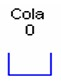
\includegraphics[width=0.15\textwidth]{Imagen 7.jpeg}
    \caption{}
    \label{fig:mi_imagen}
\end{figure}

En la cola se almacenan los ítems que están haciendo fila. Al hacer doble clic sobre ésta se observa: 

\begin{figure}[H]
    \centering
    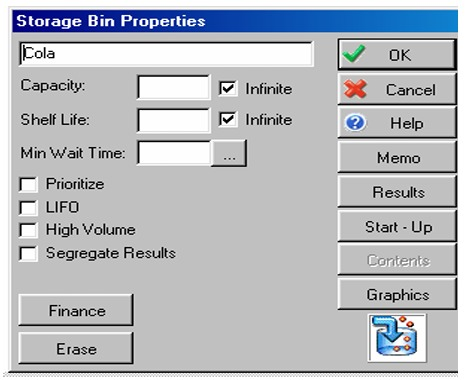
\includegraphics[width=0.5\textwidth]{Imagen 8.jpeg}
    \caption{}
    \label{fig:mi_imagen}
\end{figure}

- \textbf{Capacidad}: Si la cola tiene una capacidad limitada, aquí se debe especificar cual es la máxima capacidad.  \\

- \textbf{Shelf life}: Esta opción se emplea cuando los ítems no deben permanecer en la cola más de cierto tiempo. Es el tiempo máximo en cola. Si se pasa del tiempo, el ítem se puede dañar. \\

- \textbf{Min Wait time}: Tiempo mínimo de espera, se usa para hacer esperar al ítem cierto tiempo en cola. En algunos procesos se requiere un tiempo de almacenamiento para lo cual la cola funcionaría como un centro de trabajo. \\ 

- \textbf{Segregate Results}:Categoriza los resultados, los cuales se pueden dividir para analizarlos por separado. Se usa un label.   

Normalmente los ítems llegan al final de la cola y esperan hasta llegar al inicio, a menos que:  

- El tiempo Shelf Life se haya pasado, por lo que los ítems salen Al Work Center que trabaja con los ítems  “expirados”.

-Se haya seleccionado la opción de Prioritize, donde los ítems no llegan al final sino que dependiendo de la prioridad pasan al inicio de la cola. Esta prioridad se da con labels. Mientras mayor sea el valor del label mayor será la prioridad.

-Se seleccione la regla LIFO: último en entrar, primero en salir. \\

- \textbf{Resultados}: Muestra medidas de desempeño importantes en el análisis del sistema. \\

- \textbf{Contenido}: Permite observar los detalles de los ítems que están actualmente en la cola.  \\

- \textbf{Start up}: Si se desea que al iniciar la simulación haya ítems en cola, se debe especificar la cantidad y el tipo de work ítem.  \\

- \textbf{Gráficos}:

\begin{figure}[H]
    \centering
    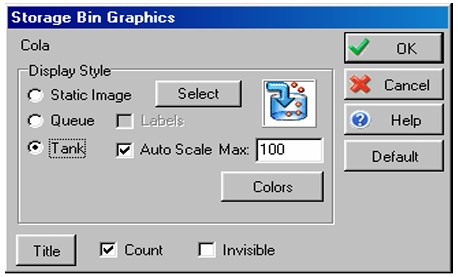
\includegraphics[width=0.5\textwidth]{Imagen 9.jpeg}
    \caption{}
    \label{fig:mi_imagen}
\end{figure}

Hay varias opciones para el gráfico de la cola: \\

- Queue: muestra los ítems que están en fila. 

- Tank: muestra una especie de tanque que se va llenando. \\

Para que se vea el titulo, en “title”, se selecciona la opción “show title...”  

\subsubsection{CENTRO DE TRABAJO (WORK CENTER)} La imagen es: 

\begin{figure}[H]
    \centering
    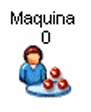
\includegraphics[width=0.15\textwidth]{Imagen 10.jpeg}
    \caption{}
    \label{fig:mi_imagen}
\end{figure}

Un Centro de trabajo es el lugar o estación donde se le realiza el trabajo al ítem. Al hacer doble clic sobre él, se observa el cuadro: 

\begin{figure}[H]
    \centering
    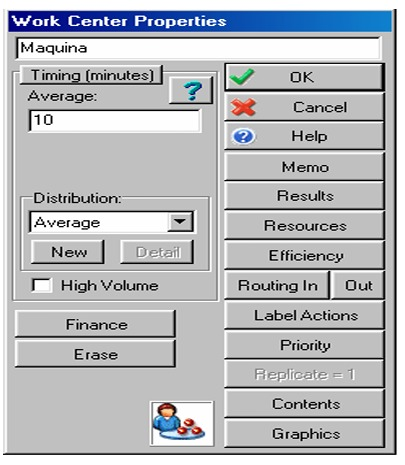
\includegraphics[width=0.5\textwidth]{Imagen 11.jpeg}
    \caption{}
    \label{fig:mi_imagen}
\end{figure}

- \textbf{Timing}: El tiempo que el centro de trabajo se demore para realizar su labor es determinado por la distribución de servicio. Ésta se selecciona del timing box. Al seleccionar la distribución se deben introducir los parámetros requeridos. La distribución puede ser cualquiera de la lista o se puede crear una nueva (New).   \\

- \textbf{Resources} (Recursos): Algunos centros de trabajo requieren de un recurso (operario) para poder realizar su labor, que en ocasiones es compartido con otros centros. En “resource” se debe determinar cuál es el recurso que se necesita.  \\

- \textbf{Resultados}: Contiene las medidas de desempeño a adicionar.  
Eficiencia: permite especificar la tasa de eficiencia con que trabaja el centro de trabajo. Esta eficiencia está relacionada con los daños o paros. Contiene las opciones:  \\

- Auto: Sirve para determinar rápidamente la eficiencia. Simul8 utiliza una distribución típica para generar paros.

- Detallada: Se pude especificar con distribuciones, el tiempo entre paros, el tiempo que dura la reparación y el tipo de paro.  \\

- \textbf{Routing In} (Ruta de Entrada): Describe cómo llega el ítem al Work Center. Hay varias disciplinas:  \\

- Priority: Esta disciplina de llegada toma el ítem que esté en el tope de la lista de ítems disponibles. 

- Collect: Un número específico de ítems es recolectado de la lista de objetos. Cada grupo recolectado se convierte en un solo ítem en el centro de trabajo (ej: ensambles). Cuando se tengan todos los ítems necesarios, se empieza el trabajo, antes no. 

- Passive: Acepta un ítem empujado desde otros objetos. No hala los ítems como lo haría normalmente.

- Expired only: Solo acepta un work ítem cuyo “shelf life” haya expirado. 

- Oldest: Hala el ítem que haya esperado más tiempo.

- Youngest: Hala el ítem que haya esperado menos tiempo.  

- Longest: Hala ítems de la cola más larga.  

- Circulate: El primer ítem es tomado de la primera entrada en la lista, el segundo de la segunda entrada y así sucesivamente. 

- Locked:Bloquea la entrada. \\

- \textbf{Routing out}: Las disciplinas de salida funcionan igual que las explicadas en la entrada. La diferencia es que el Work Center se puede programar en el Visual Logic: cuando el trabajo este completo, antes de que salga y en la salida. \\

- \textbf{Label action}: Se utiliza cuando se esta trabajando con atributos. \\

- \textbf{Priority}: Cuando dos o más centros de trabajo están compitiendo por un mismo recurso, el Work Center que tenga mayor prioridad es el que “gana” el recurso, cuando esté disponible. Por defecto la prioridad es 50 y es igual en todos los W.C.  \\

\textbf{Contents}: Permite observar los detalles de los ítems que están actualmente en el Centro de trabajo. \\

- \textbf{Gráficos}: Permite cambiar el gráfico del work center. Tiene la opción de cambiar la imagen cuando este está: trabajando, bloqueado, parado y cambiando (change over). 

\subsubsection{SALIDA (WORK COMPLETE)} La imagen es: 

\begin{figure}[H]
    \centering
    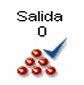
\includegraphics[width=0.15\textwidth]{Imagen 12.jpeg}
    \caption{}
    \label{fig:mi_imagen}
\end{figure}

Por esta sale el ítem completado del modelo. Al hacer doble clic sobre ella, se despliega el siguiente cuadro: 

\begin{figure}[H]
    \centering
    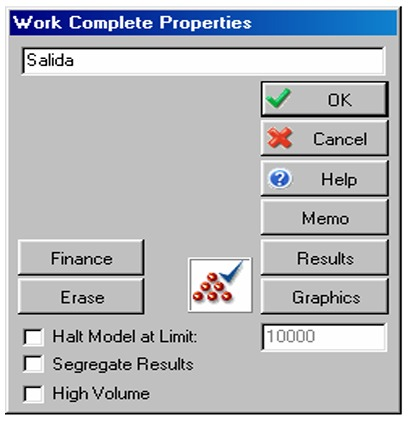
\includegraphics[width=0.5\textwidth]{Imagen 13.jpeg}
    \caption{}
    \label{fig:mi_imagen}
\end{figure}

- \textbf{Halt model at limit}: Esta opción permite que el modelo pare cuando cierto número de trabajos se ha procesado. \\

- \textbf{Segregate Results}: Categoriza los resultados. Los resultados se pueden dividir para analizarlos por separado. Se usa un label. \\

- \textbf{Resultados}: Muestra las medidas de desempeño importantes para el modelo.  \\

- \textbf{Gráficos}: Para que se vea el titulo, en “title”, se selecciona la opción “show title...” \\

\subsubsection{RECURSO (RESOURCE)}: 

\begin{figure}[H]
    \centering
    
\includegraphics[width=0.15\textwidth]{Imagen 14.jpeg}
    \caption{El recurso puede ser requerido para procesar los trabajos o para la reparación de la máquina.}
    \label{fig:mi_imagen}
\end{figure}

\subsubsection{FLECHAS}: 

\begin{figure}[H]
    \centering
    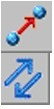
\includegraphics[width=0.15\textwidth]{Imagen 15.jpeg}
    \caption{\\ 1. Sirve para conectar los objetos. \\ 2. Al activar esta opción se pueden ver las flechas del modelo.}
    \label{fig:mi_imagen}
\end{figure}

\subsubsection{RESULTADOS}: 

\begin{figure}[H]
    \centering
    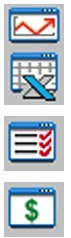
\includegraphics[width=0.15\textwidth]{Imagen 16.jpeg}
    \caption{\\ 1. Esta opción construye graficas de tiempo de los objetos seleccionados. \\  2. Muestra la información en una hoja de cálculo. \\ 3. Este es el “Results Summary”. Aquí aparecen los resultados de interés, seleccionados por el usuario al final de la corrida. Cuando se corre varias veces el modelo (multiple runs) aparecen los intervalos de confianza. \\ 4.  Muestra un informe financiero de la simulación (esto no se va a trabajar en el curso).}
    \label{fig:mi_imagen}
\end{figure}

\subsubsection{EJEMPLO}: 

\begin{figure}[H]
    \centering
    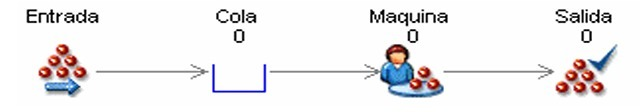
\includegraphics[width=0.65\textwidth]{Imagen 17.jpeg}
    \caption{}
    \label{fig:mi_imagen}
\end{figure}





\end{document}
